\documentclass{article}
\usepackage{graphicx}

\title{Chapter 4}
\author{Nurul Kamila (1184038) }
\date{November 2019}

\begin{document}

\maketitle

\section{Teori}
\begin{enumerate}
    \item Apa itu fungsi file CSV, jelaskan sejarah dan contoh \\
    Format file csv Comma Separated Values yaitu suatu format data pada basis data dimana setiap record yang dapat dipisahkan dengan menggunakan tanda koma (‘,’) atau juga bisa dengan menggunakan titik koma (‘;’) sebagai tanda pemisah antara datu elemen dengan elemen yang lainnya. Selain bahasa programnya yang sederhana, format ini juga dapat dibuka dengan menggunakan berbagai text-editor seperti Notepad, Wordpad, dan MS Excel. \\
    \\
   \textbf{ Sejarah file CSV}\\
   IBM Fortran (level H extended) compiler di bawah OS/360 mendukung fomat CSV pada tahun 1972. FORTRAN 77 mendefinisikan penulisannya dimana input atau output menggunakan tanda koma atau spasi untuk pembatas antar data dan penulisan tersebut sudah disetujui pada tahun 1978. Osborne Executive computer yang mengembangkan SuperCalc spreadsheet pada tahun 1983 membuat konvensi kutipan CSV yang memungkinkan string mengandung koma. Inisiatif standardisasi utama mentransformasi ¨definisi fuzzy defactom¨enjadi definisi yang lebih tepat dan de jure adalah pada tahun 2005, dengan RFC4180, mendefinisikan CSV sebagai Tipe Konten MIME. Kemudian, pada tahun 2013, beberapa kekurangan RFC4180 ditangani oleh rekomendasi W3C. Pada 2014 IETF menerbitkan RFC7111 yang menjelaskan aplikasi fragmen URI pada dokumen CSV. RFC7111 menentukan bagaimana rentang baris, kolom, dan sel dapat dipilih dari dokumen CSV menggunakan indeks posisi. Pada 2015 W3C, dalam upaya meningkatkan CSV dengan semantik formal, mempublikasikan draftrekomendasi pertama untuk stadar metadata CSV, yang dimulai sebagai rekomendasi pada bulan Desembertahun yang sama.\\
   \\
  \textbf{ Contoh:}\\
  \begin{center}
    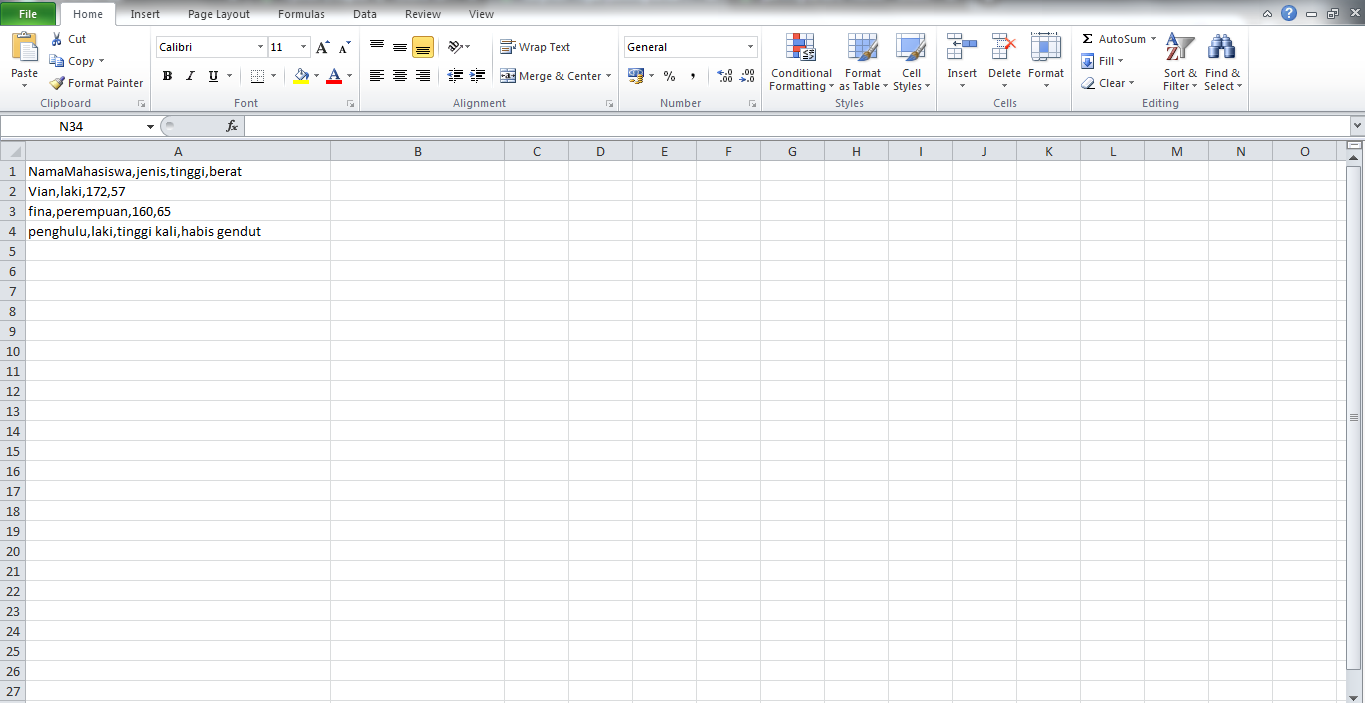
\includegraphics[width=.8\textwidth]{1.PNG}
    \end{center}

    \item Aplikasi untuk Membuat File CSV\\
    Berikut merupakan aplikasi-aplikasi yang dapat membuat file csv; Google sheet, Ms.Excel, Notepad, Numbers (MacOS), Wordpad,dll.
    
    \item Cara Membaca dan Menulis File CSV di Excel atau Spreadsheet\\
     1. Membuka aplikasi excel\\
     2. K adalah kolom dan B adalah baris\\
     3. Kemudian K1 dan B1 di isi dengan Npm, K1 dan B2 di isi dengan Nama, K1 dan B2 di isi dengan Kelas \\
     4. Kemudian pada baris ke selanjutnya adalah ricord\\
     \begin{center}
    \includegraphics[width=.8\textwidth]{1-1.PNG}
    \end{center}
     5. Selanjutnya jika telah seperti atas maka selanjutnya kita save as dan pada save as type kita ganti jadi csv (Comman delimited)\\
     5. Maka akan file csv telah dibuat\\
     \begin{center}
    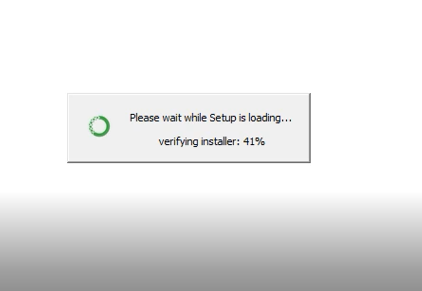
\includegraphics[width=.8\textwidth]{2.PNG}
    \end{center}
     
     \item  Sejarah library csv \\
     Library csv mengimplementasikan kelas yang digunakan untuk membaca dan menulis data dalam format csv. Ini memungkinkan programmer untuk mengatakan ”baca data dari file ini yang dihasilkan oleh Excel”. Pemrogram juga bisa menentukan format csv sesuai dengan keinginan mereka sendiri.
     
     \item  sejarah library pandas\\
     Pengembangan pandas dumulai pada tahun 2008 di AQR Captal Management. Pandas pada akhir 2009 telah menjadi open source dan secara aktif didukung oleh komunitas individu yang berpikiran sama di seluruh indonesia yang menyumbangkan waktu dan energi mereka untuk membuat pandas bersifat open source mnjadi mungkin. Pandas adalah proyek yang di sponsori oleh NumFOCUS sejak 2005. Ini akan sangat membantu untuk memastikan keberjasilan pengembangan pandas sebagi proyek sumber terbuka kelas dunia.
     
     \item Fungsi-fungsi yang terdpat pada library CSV\\
     1.  reader\\
        Fungsi ini digunakan untuk membaca isi file berformat CSV dari list.\\
        \begin{center}
    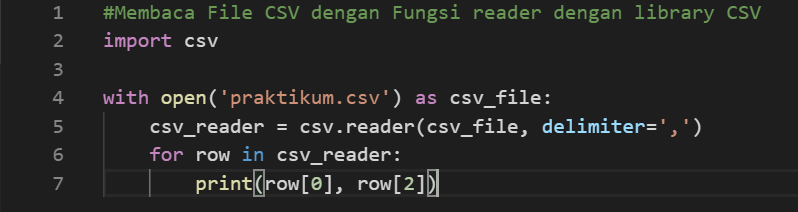
\includegraphics[width=.8\textwidth]{3.PNG}
    \end{center}
    \\
    2. DictReader\\
        Fungsi ini digunakan untuk membaca isi file berformat CSV dari dictionary.\\
        \begin{center}
    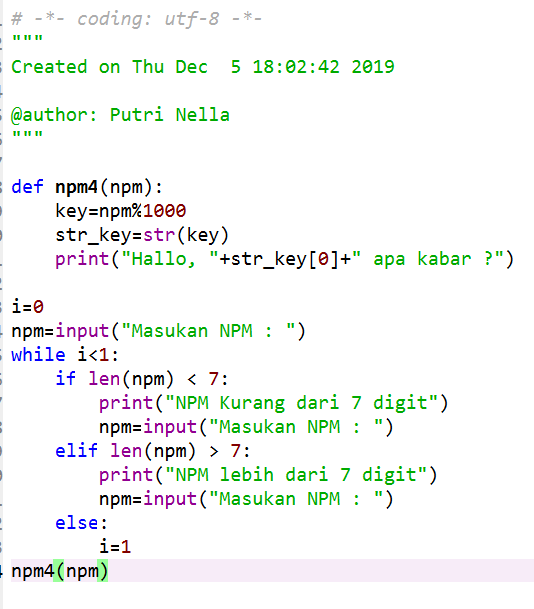
\includegraphics[width=.8\textwidth]{4.PNG}
    \end{center}
    \\
    3.  write\\
        Fungsi ini digunakan untuk menulis file berformat CSV dari list.\\
         \begin{center}
    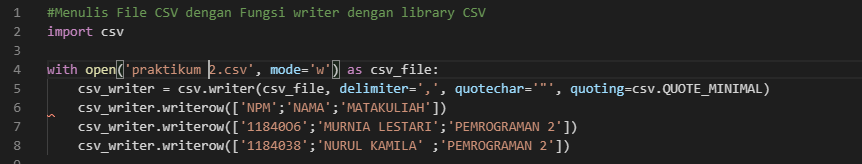
\includegraphics[width=.8\textwidth]{5.PNG}
    \end{center}
    \\
    4. DictWrite\\\
    Fungsi ini digunakan untuk menulis file berformat CSV dari dictionary.\\
    \begin{center}
    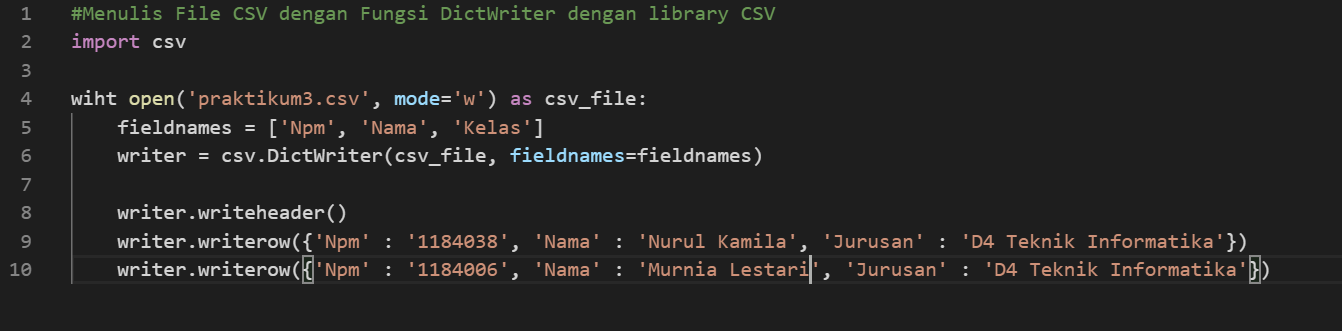
\includegraphics[width=.8\textwidth]{6.PNG}
    \end{center}
    
   \item Fungsi-fungsi yang terdpat pada library Pandas\\
   1.  Read csv\\
   Fungsi ini digunakan untuk membaca isi file berformat CSV.\\
   \begin{center}
    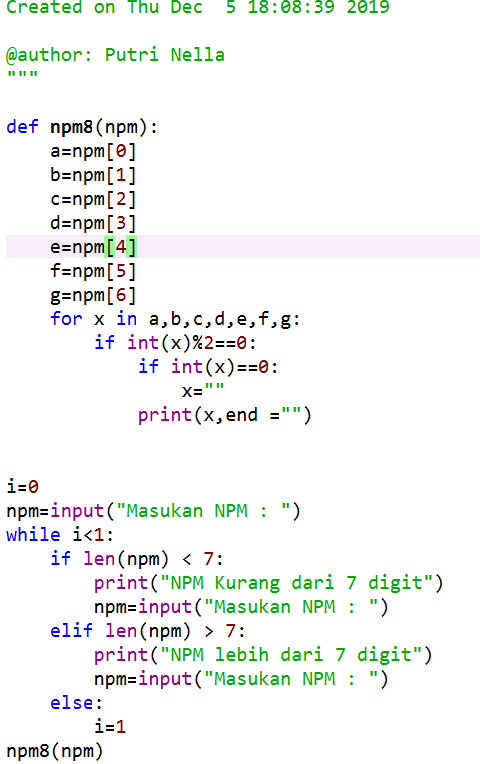
\includegraphics[width=.8\textwidth]{7.PNG}
    \end{center}
    
    2.  to csv\\
    Fungsi ini digunakan untuk menulis file berformat CSV.\\
    \begin{center}
    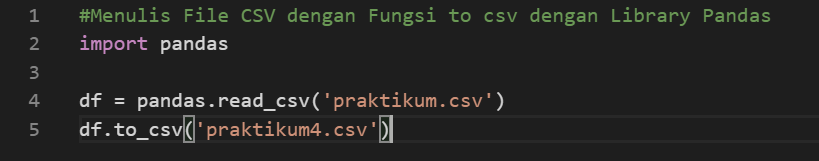
\includegraphics[width=.8\textwidth]{8.PNG}
    \end{center}
\end{enumerate}

\section{Keterampilan}
\begin{enumerate}
    \item Membuat fungsi (file terpisah/library dengan nama NPM csv.py) untuk membuka file csv dengan lib csv mode list. Berikut adalah pemanggilan file csv dengan library csv yang menggunakan list\\
    \begin{center}
    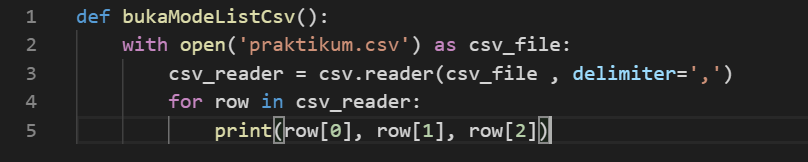
\includegraphics[width=.8\textwidth]{9.PNG}
    \end{center}
    
    \item Membuat fungsi (file terpisah/library dengan nama NPM csv.py) untuk membuka file csv dengan lib csv mode dictionary. Berikut adalah pemanggilan file csv dengan library csv yang menggunakan dictionary.\\
    \begin{center}
    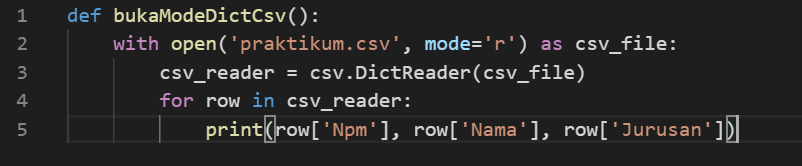
\includegraphics[width=.8\textwidth]{10.PNG}
    \end{center}
    
    \item Membuat fungsi (file terpisah/library dengan nama NPM pandas.py) untuk membuka file csv dengan lib csv mode list. Berikut adalah pemanggilan file csv dengan library pandas yang menggunakan list.\\
    \begin{center}
    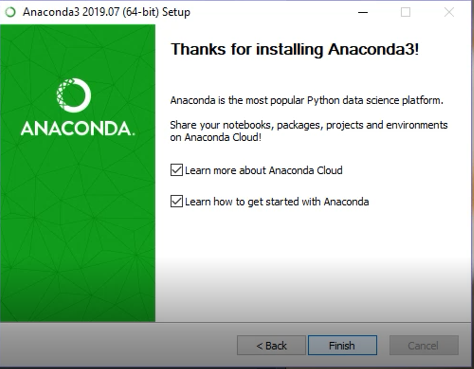
\includegraphics[width=.8\textwidth]{11.PNG}
    \end{center}
    
    \item Membuat fungsi (file terpisah/library dengan nama NPM pandas.py) untuk membuka file csv dengan lib csv mode dictionary. Berikut adalah pemanggilan file csv dengan library csv yang menggunakan dictionary.\\
    \begin{center}
    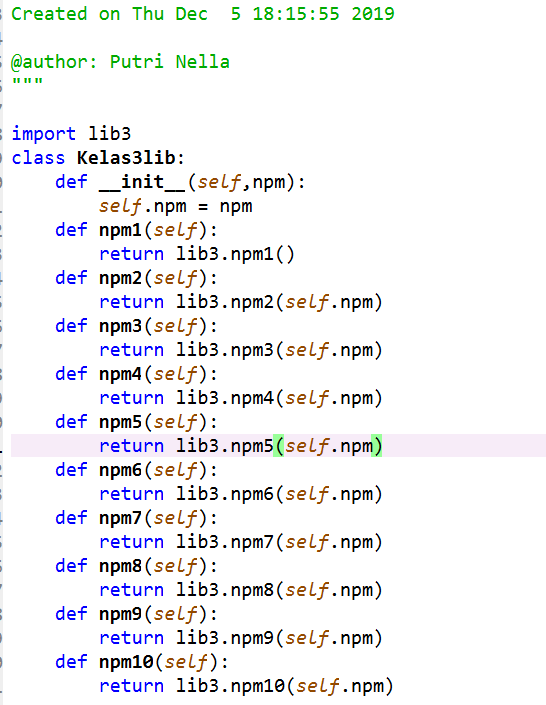
\includegraphics[width=.8\textwidth]{12.PNG}
    \end{center}
    
    \item Membuat fungsi pada file NPMpandas.py, untuk mengubah format tanggal menjadi standar dataframe. Berikut cara mengubah standar penulisan tanggal dengan mengikuti standar penulisan dari pandas.\\
    \begin{center}
    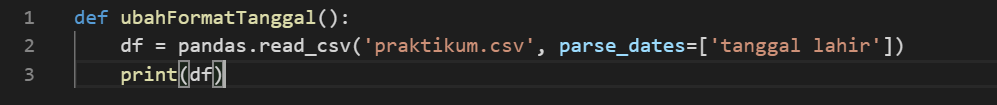
\includegraphics[width=.8\textwidth]{13.PNG}
    \end{center}
    
    \item Membuat fungsi pada file NPMpandas.py, untuk mengubah index kolom. Berikut muerpakan index kolom.\\
    \begin{center}
    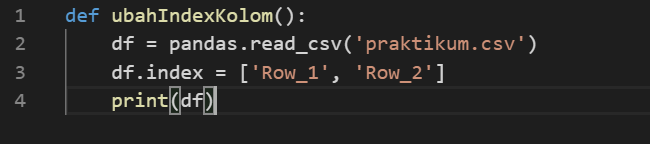
\includegraphics[width=.8\textwidth]{14.PNG}
    \end{center}
    
    \item Membuat fungsi pada file NPMpandas.py, untuk mengubah atribut atau nama kolom berikut merupakan pengguna untuk mengubah nama atibut yang digunakan, atau merubah nama header.\\
    \begin{center}
    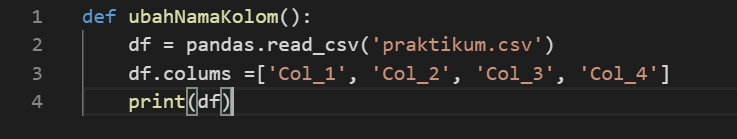
\includegraphics[width=.8\textwidth]{15.PNG}
    \end{center}
    
    \item Membuat program main.py untuk menggunakan library NPMcsv.py yang dapat membuat file dan membaca file csv.\\
    \begin{center}
    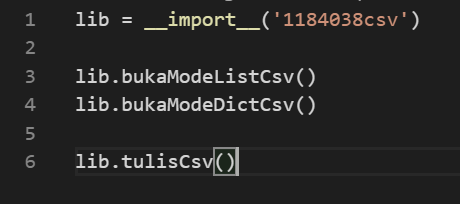
\includegraphics[width=.8\textwidth]{16.PNG}
    \end{center}
    
    \item Membuat program main.py untuk menggunakan library NPMpandas.py yang dapat membuat file dan membaca file csv.\\
    \begin{center}
    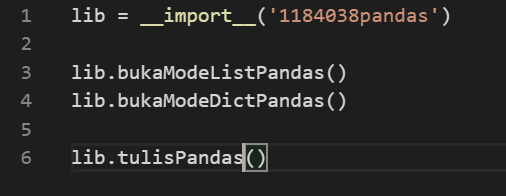
\includegraphics[width=.8\textwidth]{17.PNG}
    \end{center}
\end{enumerate}
\section{Penanganan error}
    \begin{center}
    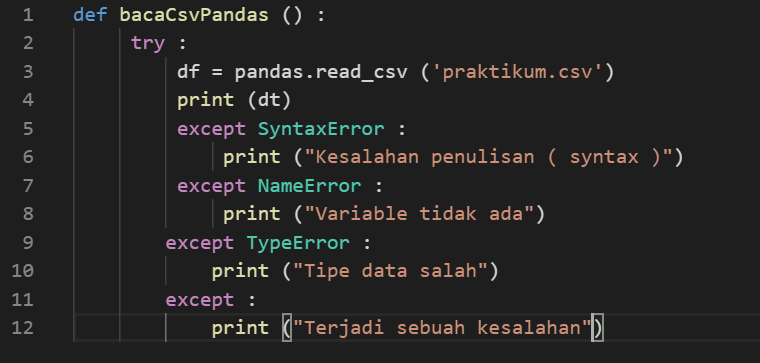
\includegraphics[width=.8\textwidth]{18.PNG}
    \end{center}
\end{document}
